% classes
\documentclass{article}

% packages
\usepackage{graphicx}
\usepackage{fancyhdr} % Required for custom headers
\usepackage{lastpage} % Required to determine the last page for the footer
\usepackage{extramarks} % Required for headers and footers
\usepackage{courier} % Required for the courier font

\usepackage{color}
\usepackage{enumitem}

\usepackage{hyperref}

\usepackage{fancyvrb}
\newenvironment{Schunk}{}{}
\DefineVerbatimEnvironment{Sinput}{Verbatim}{fontshape=sl}

\newcommand{\code}[1]{\texttt{#1}}
% \newcommand{\pkg}[1]{\mbox{\textbf{#1}}}
\newcommand{\pkg}[1]{\mbox{\texttt{#1}}}
\newcommand{\proglang}[1]{\textsf{#1}}

\usepackage[T1]{fontenc}

% page layout

\topmargin=-0.45in
\evensidemargin=0in
\oddsidemargin=0in

\textwidth=6.5in
\textheight=9.0in

\headsep=0.25in

\linespread{1.1} % Line spacing
 
\pagestyle{fancy}

% headers and footers

\fancyhf{}

\lhead{INTR 100 Breaking Intuition}

\rhead{
\includegraphics[width=0.045\textwidth]{wmlogo.jpg}}

\cfoot{Page \thepage}


% document body

\begin{document}

\vspace*{.01mm}

\begin{center}

\Large{\textcolor{blue}{\textbf{Introductory Lab.}  Some Basic Maps}}

\vspace{4mm}

\textit{Due by noon on Friday, August 28th}\\

\end{center}

\begin{figure}[h!]
\begin{center}
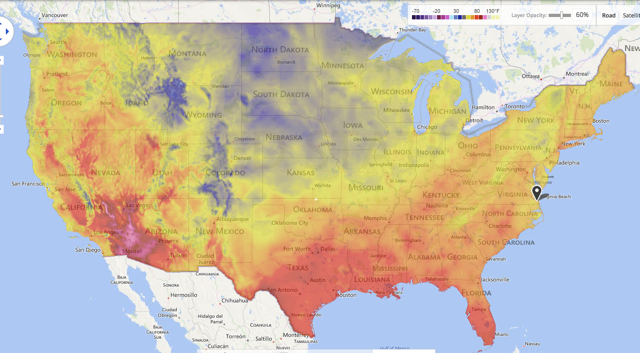
\includegraphics[width=1.0\textwidth]{weather.png}

\end{center}
\end{figure}

\setlength{\parindent}{0cm}

\large{\textit{"Everything is related to everything else, but near things are more related than distant things."}
\begin{flushright}
Tobler, 1970
\end{flushright}
}




\newpage

% Enumerate the Laboratory Objectives

\large{\textbf{Laboratory in Brief:}}

\vspace{4mm}

\setlength{\leftskip}{1cm}

\setlength{\parindent}{0cm}

The purpose of this laboratory is to ...

\vspace{4mm}

\setlength{\leftskip}{0cm}

\large{\textbf{Goals of this Laboratory:}}

\begin{enumerate}[leftmargin=15mm]

\item To learn how to install and load packages

\item To learn how to make a map using commands with an interpretive programming language

\end{enumerate}

% Enumerate the Laboratory Resources Needed

%\large{\textbf{Things to do in Preparation for this Lab:}}

%\begin{enumerate}[leftmargin=15mm]

%\item ...

%\item ...

%\item ...

%\end{enumerate}

% Step by Step Instructions for Day 1

\large{\textbf{Session 1: Wednesday, August 26th}}

\vspace{4mm}
\setlength{\leftskip}{1cm}
\textit{Step by Step Instructions: First we Acquire the Data}

\begin{enumerate}[leftmargin=15mm]

\item First lets open \proglang{R}

\item One of the most basic features of R is a package.  A package is an external source of code that can be installed into your local system that has specific features for executing a particular function.  First we need to install the package onto our local system, then we will need to load the package into our current session.  Installing the package only needs to be done one time, while loading it needs to be done each time we want to use it in \proglang{R}.  To do this first we install the package by typing the following command.

\begin{Schunk}
\begin{Sinput}
R> install.packages("ggmap", dependencies=TRUE)
\end{Sinput}
\end{Schunk}

Adding the comment in the command \code{dependencies=TRUE} will require \proglang{R} to install all the other packages \pkg{ggmap} is dependent upon in order for it to function properly.

\item Once you have installed the package \pkg{ggmap}, next you will need to load it into your current active \proglang{R} session. To do this type the following command

\begin{Schunk}
\begin{Sinput}
R> library(ggmap)
\end{Sinput}
\end{Schunk}

and your package is now active and ready for use.

\item Before we start writing code, we need to open a script file, then name and save it.  From the \proglang{R} console, under the File menu pull down, choose New Document.  Go ahead and save your document and give it a name.  We will be typing our \proglang{R} commands into our script file and then sending those commands to the \proglang{R}  console.  This enables us to save our commands for reuse over and over again, as well as to revise the code, in much the same way we might edit a paper.  To send a command from your script to the \proglang{R} console hold the \code{command} key and press \code{return} at the same time.  For starters we can type 

\begin{Schunk}
\begin{Sinput}
R>  1 + 1
\end{Sinput}
\end{Schunk}

in our script and send the command to the \proglang{R} console.

\item To start out lets make a "quick map" in R by assigning a place to a variable.  In order to do this we will use the arrow operator in \proglang{R} which is a combination of a less-than sign and a hyphen \code{\textless -}.  The arrow operator is used to assign output from a function to an object, or to write over an existing object, or parts of an existing object.  To start lets create and object by giving it a name.  Since we are going to create a map of our favourite University, I will use one of my favourite places.

\begin{Schunk}
\begin{Sinput}
R>  gt <- 'Georgia Tech'
\end{Sinput}
\end{Schunk}

To understand what we have done, simply type \code{R> gt} and have a look at the output from \proglang{R}.

\item Now lets execute our first function in \proglang{R}.  The package \pkg{ggmap} has a quick map function that takes a named object and attempts to "know" what you are interested in mapping, and then creates a map for you.

\begin{Schunk}
\begin{Sinput}
R>  qmap(gt, zoom = 14)
\end{Sinput}
\end{Schunk}

We can also play around with the qmap function by adding some other qualifying comments.

\begin{Schunk}
\begin{Sinput}

R>  qmap(gt, zoom = 13, source = "osm")
R>  qmap(gt, zoom = 15, source = "stamen", maptype = 
"watercolor", crop = FALSE)
R>  qmap(gt, zoom = 16, source = "stamen", maptype = 
"toner", crop = FALSE)

\end{Sinput}
\end{Schunk}

\item The help pages in \proglang{R} are notoriously difficult to read, but once you get the hang of them, they can be informative.  In order to find out more information about a particular function type \code{?qmap} and the help page for that function will pop up.

\item \textbf{\textit{Challenge:  Now create a map of your favourite school or University}}

\item Next we will use the \code{get\_map} function in \pkg{ggmap}.  This function works similar to the qmap function, but now we will be able to have more control over the output.  Type the following command.

\begin{Schunk}
\begin{Sinput}

R>  santos <- get_map(location = "Santos", zoom = 12)

\end{Sinput}
\end{Schunk}

Again we have created an object in \proglang{R}, although this time we have used the \code{get\_map()} function.  One important convention to understand, is when \proglang{R} programmers refer to a function, they generally refer to it with two parentheses after the function name, for example \code{get\_map()}.  You can type the name of the object \code{santos} into the \proglang{R} console, but this isn't going to be very helpful, since it will just print the data within the object.  You can look at it and see it it makes any sense to you.  Once you are finished lets use the \code{ggmap()} command to print our map of Santos, Brazil.

\begin{Schunk}
\begin{Sinput}

R>  ggmap(santos)

\end{Sinput}
\end{Schunk}

We can begin to do more with the \pkg{ggmap} package like add labels for the X and Y axis as well as give our plot a title.

\begin{Schunk}
\begin{Sinput}

R>  ggmap(santos) + labs(x = 'Longitude', y = 'Latitude') +  
ggtitle('The Home of Pele')

\end{Sinput}
\end{Schunk}

\item As before, in order to find out more information about a particular function type \code{?ggmap} and the help page for that function will pop up.

\item \textbf{\textit{Challenge:  Now create a map of your favourite place or a place you would like to visit one day.}}


\item Next, we will import a shape file and do some very basic spatial statistics on it.  To start lets install and load the \pkg{rgdal} just as we installed and loaded \pkg{ggmap}.

\begin{Schunk}
\begin{Sinput}
R> install.packages("rgdal", dependencies=TRUE)
R> library(rgdal)
\end{Sinput}
\end{Schunk}

We will also want to use a new \proglang{R} command in order to set the working directory.  The working directory is the location where \proglang{R} will look for files that are being referenced as part of a command.  While we can always specify the full path for a file, its often just easier to set the working directory in order to prevent our programming from becoming to verbose.

\begin{Schunk}
\begin{Sinput}
R> setwd("/Users/tyfrazier/workspace/work_life/WM/Teaching/
COLL_100/labs/lab1_basics")
\end{Sinput}
\end{Schunk}

\item Now lets read our shape file into \proglang{R} and create a new spatial object.  We use the \code{readOGR()} function in order to accomplish this task.  The \code{readOGR()} function takes two qualifiers the \code{den =} specifier and the \code{layer =} specifier.  The \code{dsn = } is just the name of the folder where the shape file and its supporting files are located.  The \code{layer =} qualifier is just the name of the shape file. 

\begin{Schunk}
\begin{Sinput}
R> acr <- readOGR(dsn = "data", layer = "accra")
\end{Sinput}
\end{Schunk}

This function will import the shape file named accra and create the \proglang{R} object named \code{acr}, which is simply a shortened naming convention for the capital city of Ghana.

\item Finally, we will use the \pkg{tmap} to print a few basic spatial maps that describe Accra.  Again lets install and load the package.

\begin{Schunk}
\begin{Sinput}
R> install.packages("tmap", dependencies=TRUE)
R> library(map)
\end{Sinput}
\end{Schunk}

Now we will use the \code{qtm()} function to spatially describe a variable.  One variable we can use is named \code{SLUM\_INDEX}.  So lets use it.

\begin{Schunk}
\begin{Sinput}
R> qtm(shp = acr, fill = "SLUM_INDEX", fill.palette = "-Blues")
\end{Sinput}
\end{Schunk}

We can also plot two variables side by side and compare them.  Another variable we can use gives us the number of households per enumeration area.

\begin{Schunk}
\begin{Sinput}
R> qtm(shp = acr, fill = c("SLUM_INDEX", "N_HH_POP"), fill.palette = c("Blues"), ncol = 2)
\end{Sinput}
\end{Schunk}

\end{enumerate}

\item \textbf{\textit{Challenge: Find a shape file with a spatial statistic that geographically describes a place, location or region and create a spatial map.}}

% Final Output from Laboratory

\setlength{\leftskip}{0cm}

\large{\textbf{Final Output for Submission}}

\vspace{4mm}
\setlength{\leftskip}{1cm}
\textit{Due by noon on Friday, August 28th:}
\vspace{2mm}

...  Make certain the Final Report meets the following criteria.

\begin{itemize}

\item The Final Report for this Intro Lab should include your name
\item A Map of your favorite School or University
\item A Map of your favourite place or a place you would like to visit one day
\item A Map created from a shapefile that describes a place, location or region statistically

\end{itemize}

% Grading

\setlength{\leftskip}{0cm}

\textbf{Grading}

\vspace{4mm}

\setlength{\leftskip}{1cm}

\setlength{\parindent}{0cm}

Generate 3 maps

%----------------------------------------------------------------------------------------

\end{document}